\documentclass[border=2pt]{standalone}
\usepackage{amsmath,amssymb,xcolor,tikz}
\usetikzlibrary{positioning,arrows.meta,calc,shapes.geometric,fit,backgrounds,bending}
\begin{document}
\definecolor{boxcol}{RGB}{52,86,122}%
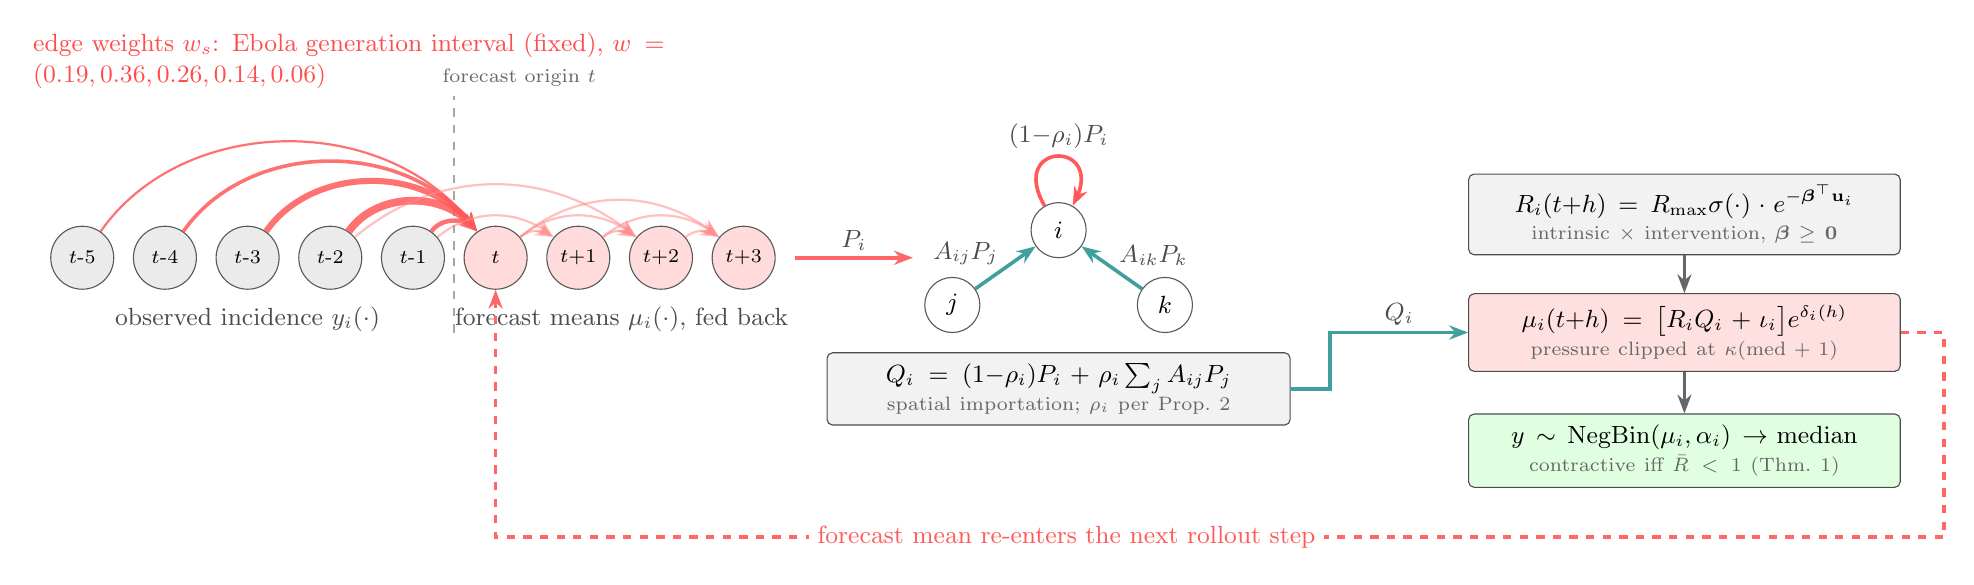
\begin{tikzpicture}[
  font=\small, x=1cm, y=1cm,
  >={Stealth[length=2.4mm]},
  rg/.style={circle, draw=black!65, fill=white, inner sep=0pt, minimum size=7mm, font=\small},
  tn/.style={circle, draw=black!65, inner sep=0pt, minimum size=8mm, font=\scriptsize},
  obs/.style={tn, fill=black!8},
  fut/.style={tn, fill=red!14},
  blk/.style={draw=black!70, rounded corners=2pt, align=center, inner sep=4pt, fill=white},
  op/.style={blk, fill=black!5, font=\small},
  f/.style={->, draw=black!60, line width=0.8pt},
  F/.style={->, draw=black!85, line width=1.3pt},
  lbl/.style={font=\small, text=black!70, inner sep=2pt},
  sub/.style={font=\scriptsize, text=black!60}
]

%% ---------------- temporal DAG ----------------
\begin{scope}[shift={(0,0)}]
  \foreach \i/\x/\lab in {1/0.0/{t\text{-}5}, 2/1.05/{t\text{-}4}, 3/2.10/{t\text{-}3}, 4/3.15/{t\text{-}2}, 5/4.20/{t\text{-}1}}
    \node[obs] (o\i) at (\x,0) {$\lab$};
  \foreach \i/\x/\lab in {1/5.25/{t}, 2/6.30/{t{+}1}, 3/7.35/{t{+}2}, 4/8.40/{t{+}3}}
    \node[fut] (p\i) at (\x,0) {$\lab$};
  \node[lbl, anchor=north] at (2.10,-0.55) {observed incidence $y_i(\cdot)$};
  \node[lbl, anchor=north] at (6.85,-0.55) {forecast means $\mu_i(\cdot)$, fed back};
  \draw[black!35, dashed, line width=0.9pt] (4.72,-0.95) -- (4.72,2.05);
  \node[sub, anchor=south] at (5.55,2.05) {forecast origin $t$};
  \foreach \s/\src/\lw in {1/o5/1.6, 2/o4/2.8, 3/o3/2.2, 4/o2/1.3, 5/o1/0.8}
    \draw[->, draw=red!65, line width=\lw pt, opacity=0.85] (\src) to[out=55,in=125] (p1);
  \foreach \a/\b in {o5/p2, o4/p3, p1/p2, p1/p3, p2/p3, p2/p4, p3/p4, p1/p4}
    \draw[->, draw=red!45, line width=0.8pt, opacity=0.55] (\a) to[out=40,in=140] (\b);
  \node[lbl, text=red!70, anchor=west, text width=86mm] at (-0.7,2.5)
    {edge weights $w_s$: Ebola generation interval (fixed), $w=(0.19,0.36,0.26,0.14,0.06)$};
\end{scope}

%% ---------------- spatial importation ----------------
\begin{scope}[shift={(12.4,0.35)}]
  \node[rg] (ri) at (0.0,0.0) {$i$};
  \node[rg] (rj) at (-1.35,-0.95) {$j$};
  \node[rg] (rk) at (1.35,-0.95) {$k$};
  \draw[F, draw=teal!75] (rj) -- node[lbl, pos=0.45, above left, inner sep=1pt] {$A_{ij}P_j$} (ri);
  \draw[F, draw=teal!75] (rk) -- node[lbl, pos=0.45, above right, inner sep=1pt] {$A_{ik}P_k$} (ri);
  \draw[F, draw=red!65] (ri) to[out=120,in=60,looseness=7] node[lbl, above, inner sep=2pt] {$(1{-}\rho_i)P_i$} (ri);
  \node[op, anchor=north, text width=56mm] (Qbox) at (0.0,-1.55)
    {$Q_i=(1{-}\rho_i)P_i+\rho_i\sum_j A_{ij}P_j$\\[-1pt]{\scriptsize\color{black!60} spatial importation; $\rho_i$ per Prop.~2}};
\end{scope}

%% ---------------- decoder blocks ----------------
\node[op, anchor=west, text width=52mm] (Rh)  at (17.6,0.55)
  {$R_i(t{+}h)=R_{\max}\sigma(\cdot)\cdot e^{-\boldsymbol{\beta}^{\top}\mathbf{u}_i}$\\[-1pt]{\scriptsize\color{black!60} intrinsic $\times$ intervention, $\boldsymbol{\beta}\!\geq\!\mathbf{0}$}};
\node[op, anchor=west, text width=52mm, fill=red!12] (muB) at (17.6,-0.95)
  {$\mu_i(t{+}h)=\big[R_iQ_i+\iota_i\big]e^{\delta_i(h)}$\\[-1pt]{\scriptsize\color{black!60} pressure clipped at $\kappa(\mathrm{med}+1)$}};
\node[op, anchor=west, text width=52mm, fill=green!12] (nbB) at (17.6,-2.45)
  {$y\sim\mathrm{NegBin}(\mu_i,\alpha_i)\rightarrow$ median\\[-1pt]{\scriptsize\color{black!60} contractive iff $\bar R<1$ (Thm.~1)}};

\draw[f] (Rh.south) -- (muB.north);
\draw[f] (muB.south) -- (nbB.north);

% P_i : temporal pressure enters the spatial graph
\draw[F, draw=red!60] (9.05,0.0) -- node[lbl, above, pos=0.5] {$P_i$} (10.55,0.0);
% Q_i : importation enters the mean  (clean elbow from the Q box)
\draw[F, draw=teal!75] (Qbox.east) -- ++(0.5,0) |- node[lbl, pos=0.75, above] {$Q_i$} (muB.west);

% forecast feedback: mean re-enters the rollout at the forecast origin
\draw[F, draw=red!60, dashed] (muB.east) -- ++(0.55,0) |- (21.1,-3.55) -- (5.25,-3.55) -- (p1.south);
\node[lbl, text=red!65, fill=white, inner sep=3pt] at (12.5,-3.55) {forecast mean re-enters the next rollout step};
\end{tikzpicture}%
\end{document}
